%!TEX root = ../main.tex
% chktex-file 46
\chapter{Learning to Aggregate on Graphs}%
\label{sec:ltag}

In the previous chapter an introduction to two separate fields of research was given:
\begin{enumerate*}
	\item \Acf{lta},
	\item \Acf{gcr}
\end{enumerate*}.
In this chapter we will combine them and define an extension of \ac{lta} to the \ac{gcr} problem.
This will be done in three steps:
\begin{enumerate}
	\item We begin with a formal definition of what actually constitutes an \ac{lta} method as opposed to non-\acs{lta} methods.
	\item Using this definition, we will see that some of the previously described \ac{gcr} methods can be interpreted as \ac{lta} variants under certain conditions.
	\item Finally a novel \acs{lta}-inspired \ac{gcnn} architecture will be described.
\end{enumerate}

\section{A Generalized Definition of \acs*{lta}}%
\label{sec:ltag:definition}

In order to formally define \ac{lta}, we must first decide on its defining characteristic.
We propose that this characteristic should be the \textit{localized explainability} of \ac{lta} predictions.
As seen in \cref{sec:related:lta}, an \ac{lta} score $y_{C} \in \mathcal{Y}$ for some multiset composition $C = \ldblbrace c_1, \dots, c_n \rdblbrace$ can always be tracked back to a set of local constituent scores $y_1, \dots, y_n \in \mathcal{Y}$.
Under the assumption that each constituent $c_i$ represents some human interpretable object, a composition's score $y_{C}$ can therefore be explained by the presence of certain indicative constituents/objects $c_i$.

Based on this intuition we now give a generalized definition of \ac{lta} which applies to unstructured as well as structured input data.
We assume that all compositions are represented by graphs $G \in \mathcal{G}$;
an unstructured input is represented by a graph with one vertex per constituent ($\mathcal{V}_G = \{ v_{c_1}, \dots, v_{c_n} \}$) and no edges ($\mathcal{E}_G = \emptyset$).
Each composition has some target score $y_G \in \mathcal{Y}$ which could be a discrete class or continuous value.
An \textit{\ac{lta} model} $h: \mathcal{G} \to \mathcal{Y}$ assigns predictions $\hat{y}_G \in \mathcal{Y}$ to compositions $G$ which ideally correspond to the true score $y_G$.
Such a model must satisfy three criteria:
\begin{enumerate}[label=\textbf{\arabic*.}]
	\item \textbf{Decomposition:}
		A given composition $G$ must be decomposed into a set of constituents $c_{G,i}$ via a \textit{decomposition function} $\psi: \mathcal{G} \to \mathcal{P}(\mathcal{G})$.
		\begin{defn}\label{defn:ltag:decomp}
			$\psi$ is a \textit{decomposition function} iff.\ it splits a graph into a subset of its subgraphs, i.e.\ $\forall G \in \mathcal{G}: \forall c_{G,i} \in \psi(G): \exists s \in \mathcal{P}(\mathcal{V}_G): c_{G,i} = G[s]$.
		\end{defn}
		Note that the strict equality $c_{G,i} = G[s]$ is used in \cref{defn:ltag:decomp} instead of just requiring subgraph isomorphism ($c_{G,i} \simeq G[s]$) because a constituent $c_{G,i}$ represents a specific localized subgraph of a structured composition.

		In the existing unstructured \ac{lta} approaches the decomposition function is implicitly defined as $\psi(G) \coloneqq {\{ G[v_{c_i}] \}}_{v_{c_i} \in \mathcal{V}_G}$ since each vertex $v_{c_i}$ corresponds to an interpretable constituent $c_i$ by definition.
		For structured data however, a split into individual vertices is typically not appropriate.
		Molecular graphs from chemical datasets for example are meaningfully characterized by the presence of so-called \textit{functional groups} consisting of multiple bonded atoms while a characterization on the level of individual atoms is generally less meaningful~\cite{McNaught1997}.
	\item \textbf{Local evaluation:}
		The constituents $c_{G, i} \in \psi(G)$ must be evaluated via some function $f: \mathcal{G} \to \mathcal{Y} \times \mathbb{R}$.
		This \textit{evaluation function} assigns a prediction $\hat{y}_{G, i} \in \mathcal{Y}$ and a weight $w_{G, i} \in \mathbb{R}$ to each constituent.
		A constituent's weight $w_{G, i}$ can intuitively be interpreted as a measure of the confidence that the local prediction $\hat{y}_{G, i}$ is indicative of the composition's global target score $y_G$.
		Learning local predictions and weights for all possible constituents is called the \textit{disaggregation problem}.

		Note that there are no explicit constituent weights in the existing unstructured \ac{lta} approaches (i.e.\ implicitly all $w_{G, i} = 1$) because the explicitly given constituents are assumed to be equally indicative of $y_G$.
		For structured data however, where the decomposition $\psi(G)$ is not given as part of the input, this assumption does not necessarily hold.
		By weighting the constituents, an \ac{lta} model can reduce the relevance or even ignore constituents that turn out to be irrelevant for the compositions target score $y_G$.
	\item \textbf{Aggregation:}
		Lastly a \textit{weighted aggregation function} $\mathcal{A}: {(\mathcal{Y} \times \mathbb{R}_{\geq 0})}^{*} \to \mathcal{Y}$ must be applied.
		It combines the multiset of local constituent predictions and non-negative weights into a single global composition prediction.
		\begin{defn}\label{defn:ltag:weighted-agg}
			We call $\mathcal{A}$ a \textit{weighted aggregation function} iff.\ it satisfies
			\begin{align*}
				\text{idempotency: } & \exists \eta > 0: \forall y \in \mathcal{Y}, w \in \mathbb{R}_{\geq 0}^n\text{ s.t. }{\max w} \geq \eta: \mathcal{A}({\ldblbrace (y, w_i) \rdblbrace}_{i=1}^n) = y \\
				\land\text{ zero invar.: } & \forall y_0 \in \mathcal{Y}, S = {\ldblbrace (y_i, w_i) \rdblbrace}_{i=1}^n: \mathcal{A}(S \cup \{ (y_0, 0) \}) = \mathcal{A}(S) \text{.}
			\end{align*}
		\end{defn}
		{\setlength{\parskip}{0pt}The idempotency constraint requires aggregation functions to agree with uniform input scores $y$ if at least one input is weighted above some threshold $\eta$.
		The zero invariance constraint requires aggregation functions to ignore inputs with zero weight.
		Exemplary weighted aggregation function are:}
		\begin{itemize}
			\item The \textit{weighted mean} function $\wmean({\ldblbrace (y_i, w_i) \rdblbrace}_{i=1}^n) \coloneqq \sum_{i=1}^n w_i y_i$ which requires $\sum w_i = 1$, $w_i \in [0, 1]$ and the existence of some scalar multiplication operator $\cdot: \mathbb{R} \times \mathcal{Y} \to \mathcal{Y}$, typically from some subfield $\mathcal{Y} \subseteq \mathbb{R}$ or possibly also some vector subspace $\mathcal{Y} \subseteq \mathbb{R}^d$.
			\item Another basic weighted aggregator is the \textit{weighted majority vote} function $\wmaj({\ldblbrace (y_i, w_i) \rdblbrace}_{i=1}^n) \coloneqq {\arg\max}_{y \in \mathcal{Y}} \sum_{y_i = y} w_i$ which returns the input with the highest total weight.
				Unlike $\wmean$ it can also be applied to score domains $\mathcal{Y}$ without a multiplication operator, e.g.\ sets of discrete classes.
			\item Alternatively an unweighted aggregation function like $\min$, $\max$, $\mean$ or \ac{owa}\footnote{
				Even though \ac{owa} uses weights, it does not get those weights as part of the input and is therefore considered to be unweighted in this context.
			} also trivially satisfies \cref{defn:ltag:weighted-agg} if all inputs $y_i$ with $w_i = 0$ are filtered out and the weights for all remaining inputs are ignored.
		\end{itemize}
\end{enumerate}
\begin{figure}[ht]
	\centering
	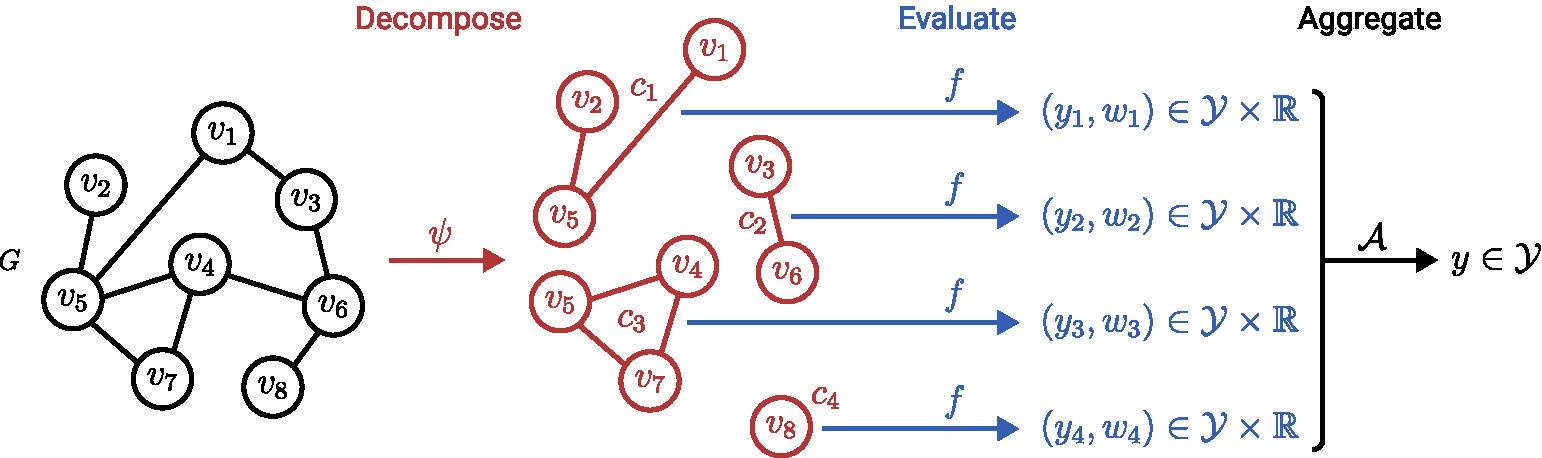
\includegraphics[width=\linewidth]{gfx/graph-lta/ltag-overview.pdf}
	\caption{
		Overview of the generalized \ac{lta} architecture for structured data.
	}\label{fig:ltag:ltag-overview}
\end{figure}
Based on the notion of decomposition, local evaluation and aggregation we can now define the concept of \textit{\ac{lta} formulations}.
\begin{defn}
	A model $h: \mathcal{G} \to \mathcal{Y}$ is in an \textit{\ac{lta} formulation} iff.\ it is expressed as
	\begin{align*}
		h(G) \coloneqq \mathcal{A}(\ldblbrace f(c_{G,i})\, |\, c_{G,i} \in \psi(G) \rdblbrace) \quad\text{with $\psi$, $f$ and $\mathcal{A}$ as defined above.}
	\end{align*}
\end{defn}
Note that every model $h: \mathcal{G} \to \mathcal{Y}$ has a trivial recursive \ac{lta} formulation by choosing $\psi(G) = \{ G \}$, $f(G) = (h(G), 1)$ and an arbitrary weighted aggregation function $\mathcal{A}$.
Those trivial \ac{lta} formulations do not split compositions into locally evaluated constituents and therefore intuitively do not fulfill the postulated localized explainability characteristic of \ac{lta}.
However since there is no commonly accepted formal criterion to decide whether a model's decisions are explainable~\cite{Lipton2018}, we do not attempt to strictly distinguish between \ac{lta} and non-\acs{lta} methods.
Instead the notion of \ac{lta} formulations should be seen as way to identify how ``\acs{lta}-like'' a model is:
\begin{itemize}
	\item \textbf{Negative extreme:}
		If a model $h$ only has trivial \ac{lta} formulations with the decomposition function $\psi(G) = \{ G \}$, it is not considered to be an \ac{lta} model.
	\item \textbf{Positive extreme:}
		If a model has an \ac{lta} formulation with a decomposition function that returns interpretable constituents, it is considered to be an \ac{lta} model.
		By definition this is true for the constituents $\psi(G) \coloneqq {\{ G[v_{c_i}] \}}_{v_{c_i} \in \mathcal{V}_G}$ of \ac{lta} methods for unstructured data.
	\item \textbf{In-between cases:}
		An \ac{lta} method for structured data must produce models that lie somewhere in-between the two extremes.
\end{itemize}

The more ``\acs{lta}-like'' a given model is, the stronger its bias towards locally explainable predictions, which in turn reduces the potential expressive power of the model.
\citet{Gilpin2018} describe this trade-off between explainability and expressive power in more detail.
When considering problem domains in which the true composition scores $y_G$ are accurately described by an \acs{lta}-like generative process, a less expressive \ac{lta}-like model could however generalize better than a more expressive non-\ac{lta} model.
This idea is captured by the so-called \textit{\ac{lta} assumption}.
\begin{defn}
	A problem domain $\mathcal{D}$ satisfies the \textit{\ac{lta} assumption} iff.\ there is an \ac{lta} method which produces models with an equal or lower out-of-sample error than the models produced by non-\acs{lta} methods for most training samples from $\mathcal{D}$.
\end{defn}
Due to the fuzziness of the class of \ac{lta} methods, the \ac{lta} assumption is naturally also a fuzzy concept.
Nonetheless evidence for its truthiness in a given domain $\mathcal{D}$ can be empirically obtained by comparing candidate \ac{lta} methods with the best known non-\ac{lta} method for $\mathcal{D}$, assuming that some cut-off condition for the required ``\ac{lta}-ness'' of an \ac{lta} method is agreed upon.

\section{\acs*{lta} Formulations of Existing \acs*{gcr} Methods}%
\label{sec:ltag:formulation}

Based on the general definition of \ac{lta} from the last section, we will now see to what extent the \ac{gcr} methods described in \cref{sec:related:gcr} can be interpreted as \ac{lta} instances.
First the relation between \acp{svm} on graph embeddings and \ac{lta} will be explored.
Then we will provide an \ac{lta} perspective on \acp{gcnn}.

\subsection{\acsp*{svm} on Graph Embeddings as \acs*{lta} Models}%
\label{sec:ltag:formulation:svm}

In \cref{sec:related:gcr:embed,sec:related:gcr:kernel} three different ways to map a given graph $G$ to a vector $\varphi(G) \in \mathbb{R}^d$ were described:
\begin{enumerate*}
	\item Fingerprint embeddings,
	\item skip-gram inspired embeddings and
	\item kernel embeddings
\end{enumerate*}.
One common way to solve the \ac{gcr} problem via those embedding vectors is to train an \ac{svm} on them.
We will now see that \acp{svm} can be interpreted as \ac{lta} models if they are trained on so-called \textit{substructure component embeddings}.
\begin{defn}\label{defn:ltag:substruct-embedding}
	A graph embedding $\varphi: \mathcal{G} \to \mathbb{N}_0^{d}$ is called a \textit{substructure component embedding} iff.\ there are decomposition functions $\psi_{\varphi, i}: \mathcal{G} \to \mathcal{P}(\mathcal{G})$ and normalization constants $\gamma_i \in \mathbb{R}$ for all embedding components $i \in [d]$ s.t.\ $\forall G \in \mathcal{G}, i \in [d]: \varphi(G)[i] = \gamma_i {| \psi_{\varphi, i}(G) |}$.
	The joint decomposition $\psi_{\varphi}(G) \coloneqq \bigcup_{i=1}^d \psi_{\varphi,i}(G)$ is a so-called \textit{underlying decomposition} of the embedding $\varphi$.
\end{defn}
Intuitively \cref{defn:ltag:substruct-embedding} states that every embedding dimension must represent the number of constituents produced by some decomposition function.
Based on this requirement we now proof the main theorem which shows the relation between \acp{svm} and \ac{lta}.

\begin{thm}\label{thm:ltag:svm-ltag-formulation}
	A binary \ac{svm} graph classifier $h$ that applies a substructure component embedding $\varphi$ to its inputs has an \ac{lta} formulation with the decomposition function $\psi_{\varphi}$.
\end{thm}
\begin{proof}
	Let $h: \mathcal{G} \to {\{ -1, +1 \}}$ be a binary graph classifier expressed as $h = h_{\text{\acs*{svm}}} \circ \varphi$ where $\varphi: \mathcal{G} \to \mathbb{N}_0^{d}$ is a substructure component embedding and $h_{\text{\acs*{svm}}}: \mathbb{R}^{d} \to {\{ -1, +1 \}}$ a standard \ac{svm} classifier.
	Additionally, let $\psi_{\varphi}$ be some underlying decomposition of $\varphi$.

	Based on this decomposition we now bring the \ac{svm} graph classifier $h$ into an \ac{lta} formulation.
	If $h$ is trained on a dataset $\mathcal{D}_{\text{train}} = {\{ (G_1, y_1), \dots, (G_N, y_N) \}}$, via the kernel trick it can be expressed as
	\begin{align*}
		h(G) &= \sgn\left( \sum_{j = 1}^{N} \alpha_j y_j {\langle \varphi(G), \varphi(G_j) \rangle} + b \right)
		\quad\text{for some $\alpha \in \mathbb{R}^N$ and $b \in \mathbb{R}$} \\
		&= \sgn\left( {\sum_{i=1}^{d} {
				\underbrace{\varphi(G)[i]}_{{|\psi_{\varphi, i}(G)|} \gamma_i^{-1}}
				\underbrace{\left( \sum_{j = 1}^{N} \alpha_j y_j {\varphi(G_j)}[i] \right)}_{\beta_i}}
			} + b \right)
		 = \sgn\left( {\sum_{i=1}^{d} {{|\psi_{\varphi, i}(G)|} \gamma_i^{-1} \beta_i}} + b \right) \\
		&= \sgn\left( {\sum_{c_t \in \psi_{\varphi}(G)} \underbrace{\sum_{i = 1}^d \mathbbm{1}[c_t \in \psi_{\varphi, i}(G)] \gamma_i^{-1} \beta_i}_{z_t}} + b \right)
		 = \sgn\left( {\sum_{c_t \in \psi_{\varphi}(G)}} \underbrace{|z_t|}_{w_t} \underbrace{\sgn{z_t}}_{y_t} + {\underbrace{|b|}_{w_b} \underbrace{\sgn{b}}_{y_b}} \right) \\
		&= \wmaj\left( \ldblbrace (y_t, w_t)\, |\, c_t \in \psi_{\varphi}(G) \rdblbrace \cup \ldblbrace (y_b, w_b) \rdblbrace \right)
		\text{.}
	\end{align*}
	By choosing $f_h(c_t) \coloneqq (y_t, w_t)$ and $\mathcal{A}_h(S) = \wmaj(S \cup \ldblbrace (y_b, w_b) \rdblbrace)$, the \ac{svm} model therefore has an \ac{lta} formulation with the decomposition function $\psi_{\varphi}$.
	To see why $\mathcal{A}_h$ satisfies \cref{defn:ltag:weighted-agg}, note that it inherits the idempotency property from $\wmaj$ because $\mathcal{A}_h$ ignores the bias ``pseudo-constituent'' $(y_b, w_b)$ for all threshold weights $\max w_t \geq \eta > w_b$, similarly the zero invariance of $\wmaj$ is also directly inherited.
	This concludes the proof.
\end{proof}

The central statement of \cref{thm:ltag:svm-ltag-formulation} is that the output of an \acs{svm}-based graph classifier can be interpreted as the weighted majority vote of constituent scores $y_t$.
Those constituent scores are in turn also the result of a weighted majority vote as shown in the following proposition.
\begin{prop}

\end{prop}

\subsection{\acsp*{gcnn} as \acs*{lta} Models}%
\label{sec:ltag:formulation:gcnn}

\section{A Novel \acs*{lta}-Inspired \acs*{gcnn} Architecture}%
\label{sec:ltag:wl2gnn}
